% Drawing 74/02-11 -- folder 74, batch 02, archive page 27 (PDF page 28).
% Transcription: trois figures de même forme, l'une sous l'autre : six groupes de trois symboles $\xi$ aux sommets d'un hexagone ; à l'intérieur, deux triangles en pointillé formant une étoile ; deux sommets voisins marqués d'un petit triangle hachuré ; en regard de chaque côté, un court trait portant une racine.
% Kind: three hexagons of triples of lines with roots on the sides (root system inside E6). Method 2 (schematic redraw from the facsimile). Status: ok.
% Notes: Three figures of one shape, one under the other, each measured on its own on the page. In each: the six triples of xi round a hexagon (labels as the transcription reads them, placed where they stand); inside, a star of two triangles whose sides are dashed or solid strokes as on the page, some broken and not all meeting (in the first figure the lower sides of the down-pointing triangle are solid; in the third the left side of the up-pointing triangle, the right part of the middle line and two lower sides are solid); two neighbouring corners carry a small triangle, hatched (upper right and lower right in the first figure, hatched vertically for the second; at the top hatched horizontally and at the upper right filled in the second; at the top cross-hatched and at the upper right filled in the third); beside each side of the hexagon a short stroke with its root, where the page writes one (no label beside the left stroke of the first figure); in the first figure the braces above the top triple and under the bottom triple. Left out: the rest of the formula r_456 = 3(r_1 + r_2 + r_3) + 2r_4 + r_5 + r_6 beside the first figure (written « r_456 = ... ») and the commutators in the right margin (text). Overlaid 2026-11-12 (Opus 5.5) on a 400 dpi colour render: the earlier redraw was one template measured on the first figure and copied, regular and closed, into the other two, 3 to 6 units off the page, with the hatched marks misplaced and a label « -r_456 » that the page does not write; all three figures redrawn from the page. Redrawn 2026-11-12 (issue 128): to check again.
% Coordinates: 1 unit = 1 mm = 1/100 of the crop width (bbox in page fractions: [0.25, 0.085, 0.62, 0.65]).
% Redrawn by Claude (claude-fable-5-2), issue #128, 2026-11-12; not checked by a human; not compiled (no TeX in the session).
% Overlaid by Claude (claude-opus-5-5) 2026-11-12 (issue #128): rasterised from its own coordinates over the colour facsimile and checked or corrected. Not compiled. Status: ok.
% Rights: reproduces part of the work -- behind RENDER_TRANSCRIPTS, never published by itself.
\documentclass[tikz,border=3pt]{standalone}
\usepackage{amsmath,amssymb}
\usetikzlibrary{patterns,arrows.meta}
\tikzset{pencil/.style={black!45}, struck/.style={black!35}, mpt/.style={circle,draw,inner sep=1.3pt}, pt/.style={circle,fill,inner sep=0.9pt}, opt/.style={circle,draw,fill=white,inner sep=1.1pt}}
\begin{document}
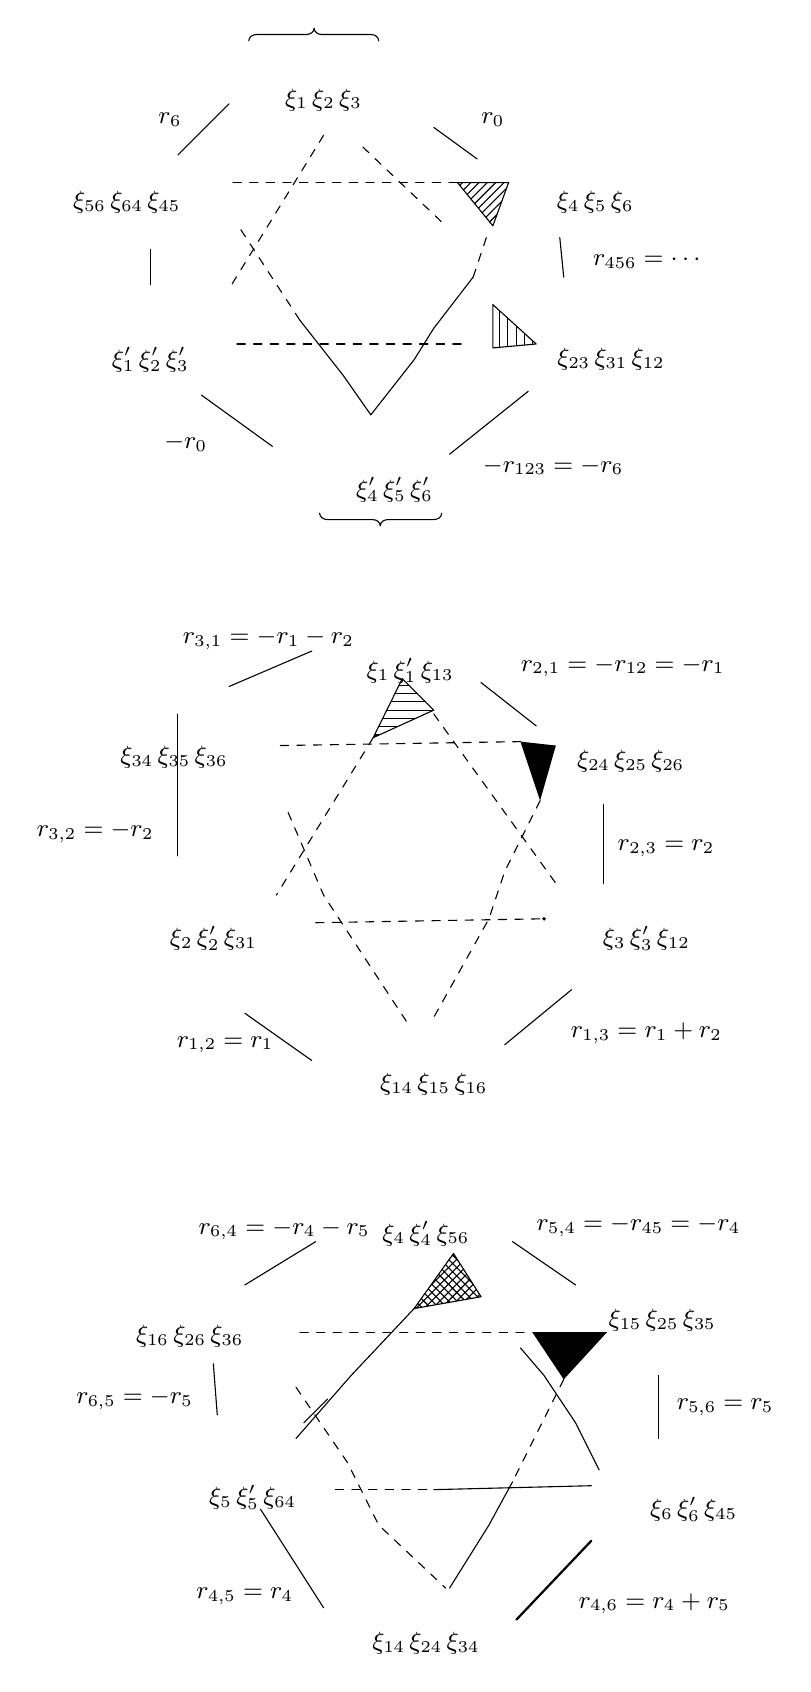
\begin{tikzpicture}[x=1mm,y=1mm,line cap=round,line join=round,font=\small]
% first figure
\node at (41,-12) {\small $\xi_{1}\,\xi_{2}\,\xi_{3}$};
\node at (75.5,-25) {\small $\xi_{4}\,\xi_{5}\,\xi_{6}$};
\node at (77.5,-45) {\small $\xi_{23}\,\xi_{31}\,\xi_{12}$};
\node at (50,-61.5) {\small $\xi_4'\,\xi_5'\,\xi_6'$};
\node at (19,-45) {\small $\xi_1'\,\xi_2'\,\xi_3'$};
\node at (16,-25) {\small $\xi_{56}\,\xi_{64}\,\xi_{45}$};
\draw (31.5,-4.5) to[out=90,in=180] (32.5,-3.7) -- (38.8,-3.7) to[out=0,in=-90] (39.8,-2.9) to[out=-90,in=180] (40.8,-3.7) -- (47,-3.7) to[out=0,in=90] (48,-4.5);
\draw (40.5,-64.5) to[out=-90,in=180] (41.5,-65.3) -- (47.2,-65.3) to[out=0,in=90] (48.2,-66.1) to[out=90,in=180] (49.2,-65.3) -- (55,-65.3) to[out=0,in=-90] (56,-64.5);
\draw[dashed] (29.5,-22.5) -- (58,-22.5);
\draw[dashed] (30.5,-28.5) -- (38,-40);
\draw (38,-40) -- (43.5,-47) -- (47,-52);
\draw (47,-52) -- (52.5,-45) -- (55,-41) -- (60,-34.5);
\draw[dashed] (60,-34.5) -- (62,-28.5);
\draw[dashed] (41,-16.5) -- (29,-36);
\draw[dashed] (46,-18) -- (56,-27.5);
\draw[dashed] (30,-43) -- (58.5,-43);
\draw[pattern=north east lines] (58,-22.5) -- (64.5,-22.5) -- (62.5,-28) -- cycle;
\draw[pattern=vertical lines] (62.5,-38) -- (62.5,-43.5) -- (68,-43) -- cycle;
\draw (22.5,-19) -- (29,-12.5);
\node at (21.5,-14.5) {\small $r_6$};
\draw (55,-15.5) -- (60.5,-19.5);
\node at (62.5,-14.5) {\small $r_0$};
\draw (71,-29.5) -- (71.5,-34.5);
\node[right] at (74,-32.5) {\small $r_{456} = \cdots$};
\draw (57,-57) -- (67,-49);
\node[right] at (60,-58.5) {\small $-r_{123} = -r_6$};
\draw (25.5,-49.5) -- (34.5,-56);
\node at (23.5,-55.5) {\small $-r_0$};
\draw (19,-31) -- (19,-35.5);
% second figure
\node at (52,-84.5) {\small $\xi_1\,\xi_1'\,\xi_{13}$};
\node at (80,-96) {\small $\xi_{24}\,\xi_{25}\,\xi_{26}$};
\node at (82,-118.5) {\small $\xi_3\,\xi_3'\,\xi_{12}$};
\node at (55,-137) {\small $\xi_{14}\,\xi_{15}\,\xi_{16}$};
\node at (27,-118.5) {\small $\xi_2\,\xi_2'\,\xi_{31}$};
\node at (22,-95.5) {\small $\xi_{34}\,\xi_{35}\,\xi_{36}$};
\draw[pattern=horizontal lines] (47.3,-93) -- (51,-85.5) -- (55,-89.5) -- cycle;
\fill (66,-93.5) -- (70.5,-94) -- (68.5,-101) -- cycle;
\draw[dashed] (35.5,-94) -- (66,-93.5);
\draw[dashed] (47.3,-93) -- (35,-113);
\draw[dashed] (55,-90) -- (70.5,-111.5);
\draw[dashed] (40,-116.5) -- (69,-116);
\draw[dashed] (36.5,-102.5) -- (41,-113) -- (51.5,-129);
\draw[dashed] (68.5,-101) -- (64,-110) -- (62,-116) -- (55,-128.5);
\node[pt,inner sep=0.5pt] at (69,-116) {};
\draw (29,-86.5) -- (39.5,-82);
\node at (34,-80.5) {\small $r_{3,1} = -r_1 - r_2$};
\draw (61,-86) -- (68,-91.5);
\node at (79,-84) {\small $r_{2,1} = -r_{12} = -r_1$};
\draw (76.5,-101.5) -- (76.5,-111.5);
\node at (84.5,-107) {\small $r_{2,3} = r_2$};
\draw (64,-132) -- (72.5,-125);
\node at (82,-130.5) {\small $r_{1,3} = r_1 + r_2$};
\draw (31,-128) -- (39.5,-134);
\node at (28.5,-132) {\small $r_{1,2} = r_1$};
\draw (22.5,-90) -- (22.5,-108);
\node at (12,-105) {\small $r_{3,2} = -r_2$};
% third figure
\node at (54,-156) {\small $\xi_4\,\xi_4'\,\xi_{56}$};
\node at (84,-167) {\small $\xi_{15}\,\xi_{25}\,\xi_{35}$};
\node at (88,-191) {\small $\xi_6\,\xi_6'\,\xi_{45}$};
\node at (54,-208) {\small $\xi_{14}\,\xi_{24}\,\xi_{34}$};
\node at (32,-189.5) {\small $\xi_5\,\xi_5'\,\xi_{64}$};
\node at (24,-169) {\small $\xi_{16}\,\xi_{26}\,\xi_{36}$};
\draw[pattern=crosshatch] (52.5,-165.5) -- (57.5,-158.5) -- (61,-164) -- cycle;
\fill (67.5,-168.5) -- (77,-168.5) -- (71.5,-174.5) -- cycle;
\draw[dashed] (38,-168.5) -- (67.5,-168.5);
\draw (52.5,-165.5) -- (44.5,-174) -- (37.5,-182);
\draw (38.5,-180) -- (41.5,-177);
\draw[dashed] (42.5,-188.5) -- (55,-188.5);
\draw (55,-188.5) -- (75,-188);
\draw (66,-170.5) -- (69,-174) -- (73,-180) -- (76,-186);
\draw[dashed] (37.5,-175.5) -- (44,-185) -- (48,-193) -- (56.5,-201);
\draw[dashed] (71.5,-174.5) -- (65,-187.5);
\draw (65,-187.5) -- (62,-193) -- (57,-201);
\draw (31,-162.5) -- (40,-157);
\node at (36,-155.5) {\small $r_{6,4} = -r_4 - r_5$};
\draw (65,-157) -- (73,-162.5);
\node at (81,-155) {\small $r_{5,4} = -r_{45} = -r_4$};
\draw (83.5,-174) -- (83.5,-182);
\node at (92,-178) {\small $r_{5,6} = r_5$};
\draw[thick] (65.5,-205) -- (75,-195);
\node at (83,-203) {\small $r_{4,6} = r_4 + r_5$};
\draw (33,-191) -- (41,-203.5);
\node at (31,-202) {\small $r_{4,5} = r_4$};
\draw (27,-172.5) -- (27.5,-179);
\node at (17,-177) {\small $r_{6,5} = -r_5$};
\end{tikzpicture}
\end{document}
